\section{AND and OR as subtraction and addition}

\subsection{ZX Spectrum ROM text strings}
\label{ZX Spectrum}

Those who once investigated ZX Spectrum \ac{ROM} internals, probably noticed that the last symbol of each text string is seemingly
absent.

\begin{figure}[H]
\centering
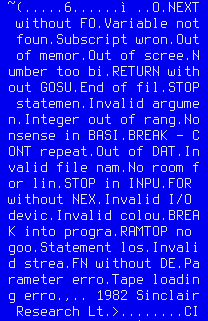
\includegraphics[width=0.3\textwidth]{fundamentals/zx_spectrum_ROM.png}
\caption{Part of ZX Spectrum ROM}
\end{figure}

There are present, in fact.

Here is excerpt of ZX Spectrum 128K ROM disassembled:

\lstinputlisting{fundamentals/ZX_Spectrum_ROM.lst}
( \url{http://www.matthew-wilson.net/spectrum/rom/128_ROM0.html} )

Last character has most significant bit set, which marks string end.
Presumably, it was done to save some space?
Old 8-bit computers has very tight environment.

Characters of all messages are always in standard 7-bit \ac{ASCII} table,
so it's guaranteed 8th bit is never used for characters.

To print such string, we must check \ac{MSB} of each byte, and if it's set, we must clear it, then print character,
and then stop.
Here is a C example:

\begin{lstlisting}[style=customc]
unsigned char hw[]=
{
	'H',
	'e',
	'l',
	'l',
	'o'|0x80
};

void print_string()
{
	for (int i=0; ;i++)
	{
		if (hw[i]&0x80) // check MSB
		{
			// clear MSB
			// (in other words, clear all, but leave 7 lower bits intact)
			printf ("%c", hw[i] & 0x7F);
			// stop
			break;
		};
		printf ("%c", hw[i]);
	};
};
\end{lstlisting}

Now what is interesting, since 8th bit is the most significant bit (in byte), we can check it, set it and remove it using
arithmetical operations instead of logical.

I can rewrite my C example:

\begin{lstlisting}[style=customc]
unsigned char hw[]=
{
	'H',
	'e',
	'l',
	'l',
	'o'+0x80
};

void print()
{
	for (int i=0; ;i++)
	{
		// hw[] must have 'unsigned char' type
		if (hw[i] >= 0x80) // check for MSB
		{
			printf ("%c", hw[i]-0x80); // clear MSB
			// stop
			break;
		};
		printf ("%c", hw[i]);
	};
};
\end{lstlisting}

By default, \IT{char} is signed type in C/C++, so to compare it with variable like 0x80 (which is negative ($-128$)
if treated as signed),
we must treat each character in text message as unsigned.

Now if 8th bit is set, the number is always larger or equal to 0x80.
If 8th bit is clear, the number is always smaller than 0x80.

Even more than that: if 8th bit is set, it can be cleared by subtracting 0x80, nothing else.
If it's not set beforehand, however, subtracting will destruct other bits.

Likewise, if 8th bit is clear, it's possible to set it by adding 0x80.
But if it's set beforehand, addition operation will destruct some other bits.

In fact, this is valid for any bit.
If the 4th bit is clear, you can set it just by adding 0x10: 0x100+0x10 = 0x110.
If the 4th bit is set, you can clear it by subtracting 0x10: 0x1234-0x10 = 0x1224.

It works, because carry isn't happened during addition/subtraction.
It will, however, happen, if the bit is already set there before addition, or absent before subtraction.

Likewise, addition/subtraction can be replaced using OR/AND operation if two conditions are met:
1) you want to add/subtract by a number in form of $2^n$;
2) this bit in source value is clear/set.

For example, addition of 0x20 is the same as ORing value with 0x20 under condition that this bit is clear before:
0x1204|0x20 = 0x1204+0x20 = 0x1224.

Subtraction of 0x20 is the same as ANDing value with ~0x20 (0x....FFDF), but if this bit is set before:
0x1234\&(\~{}0x20) = 0x1234\&0xFFDF = 0x1234-0x20 = 0x1214.

Again, it works because carry not happened when you add $2^n$ number and this bit isn't set before.

This property of boolean algebra is important, worth understanding and keeping it in mind.

